\documentclass[journal]{IEEEtran}
\usepackage[a5paper, margin=10mm]{geometry}
%\usepackage{lmodern} % Ensure lmodern is loaded for pdflatex
\usepackage{tfrupee} % Include tfrupee package


\setlength{\headheight}{1cm} % Set the height of the header box
\setlength{\headsep}{0mm}     % Set the distance between the header box and the top of the text


%\usepackage[a5paper, top=10mm, bottom=10mm, left=10mm, right=10mm]{geometry}

%
\setlength{\intextsep}{10pt} % Space between text and floats

\makeindex


\usepackage{cite}
\usepackage{amsmath,amssymb,amsfonts,amsthm}
\usepackage{algorithmic}
\usepackage{graphicx}
\usepackage{textcomp}
\usepackage{xcolor}
\usepackage{txfonts}
\usepackage{listings}
\usepackage{enumitem}
\usepackage{mathtools}
\usepackage{gensymb}
\usepackage{comment}
\usepackage[breaklinks=true]{hyperref}
\usepackage{tkz-euclide} 
\usepackage{listings}
\usepackage{multicol}
\usepackage{xparse}
\usepackage{gvv}
%\def\inputGnumericTable{}                                 
\usepackage[latin1]{inputenc}                                
\usepackage{color}                                            
\usepackage{array}                                            
\usepackage{longtable}                                       
\usepackage{calc}                                             
\usepackage{multirow}                                         
\usepackage{hhline}                                           
\usepackage{ifthen}                                               
\usepackage{lscape}
\usepackage{tabularx}
\usepackage{array}
\usepackage{float}
\usepackage{ar}
\usepackage[version=4]{mhchem}


\newtheorem{theorem}{Theorem}[section]
\newtheorem{problem}{Problem}
\newtheorem{proposition}{Proposition}[section]
\newtheorem{lemma}{Lemma}[section]
\newtheorem{corollary}[theorem]{Corollary}
\newtheorem{example}{Example}[section]
\newtheorem{definition}[problem]{Definition}
\newcommand{\BEQA}{\begin{eqnarray}}
\newcommand{\EEQA}{\end{eqnarray}}

\theoremstyle{remark}


\begin{document}
\bibliographystyle{IEEEtran}
\onecolumn

\title{2.10.59}
\author{Josyula G S Avaneesh- EE25BTECH11030}
\maketitle


\renewcommand{\thefigure}{\theenumi}
\renewcommand{\thetable}{\theenumi}
\textbf{Question} Two adjacent sides of a parallelogram ABCD are given by $\vec{B-A}=\myvec{2\\10\\11}$ and $\vec{D-A}=\myvec{-1\\2\\2}$. The side $\vec{D-A}$ is rotated by an acute angle $\alpha$ in the plane of the parallelogram so that $\vec{D-A}$ becomes $(\vec{D-A})^|$. If $(\vec{D-A})^|$ makes a right angle with the side $\vec{B-A}$ then the cosine of the angle $\alpha$ is given by\\
\begin{enumerate}
\begin{multicols}{2}
    \item $\frac{8}{9}$
    \item $\frac{\sqrt{17}}{9}$
    \item $\frac{1}{9}$
    \item $\frac{4 \sqrt{5}}{9}$
\end{multicols}
\end{enumerate}
\textbf{Solution :} Given details:
ABCD is a parallelogram.
\begin{align}
   \vec{B-A}=\myvec{2\\10\\11}\\
   \vec{D-A}=\myvec{-1\\2\\2}
\end{align}
The side $\vec{(D-A)}^|$ is perpendicular to $\vec{B-A}$.\\
\textbf{Property:} The cosine of the angle between vector 1 and vector 2 is given by $\dfrac{{n_1}^\top n_2}{\norm{n_1}\norm{n_2}} $.\\
Since $(\vec{D-A})^|$ is perpendicular to $\vec{B-A}$,\\


Let the angle between the vectors be $\theta$.
$$\alpha+\theta=\frac{\pi}{2}$$
\begin{align}
  \cos\theta=\frac{\vec{B-A}^\top\vec{D-A}}{\norm{B-A}\norm {D-A}}\\
  \cos\theta=\frac{\myvec{2&10&11}\myvec{-1\\2\\2}}{\sqrt{225}\sqrt{9}}\\
  \cos\theta=\frac{40}{45}=\frac{8}{9}\brak{\because\sin\theta=\sqrt{1-\cos^2\theta}}\\
  \sin\theta=\sqrt{1-\frac{64}{81}}\\
  \sin\theta=\frac{\sqrt{17}}{9}
\end{align}
Since $\cos\alpha=\sin\theta=\frac{\sqrt{17}}{9}$\\
Ans. option 2

\begin{figure}[H]
    \centering
    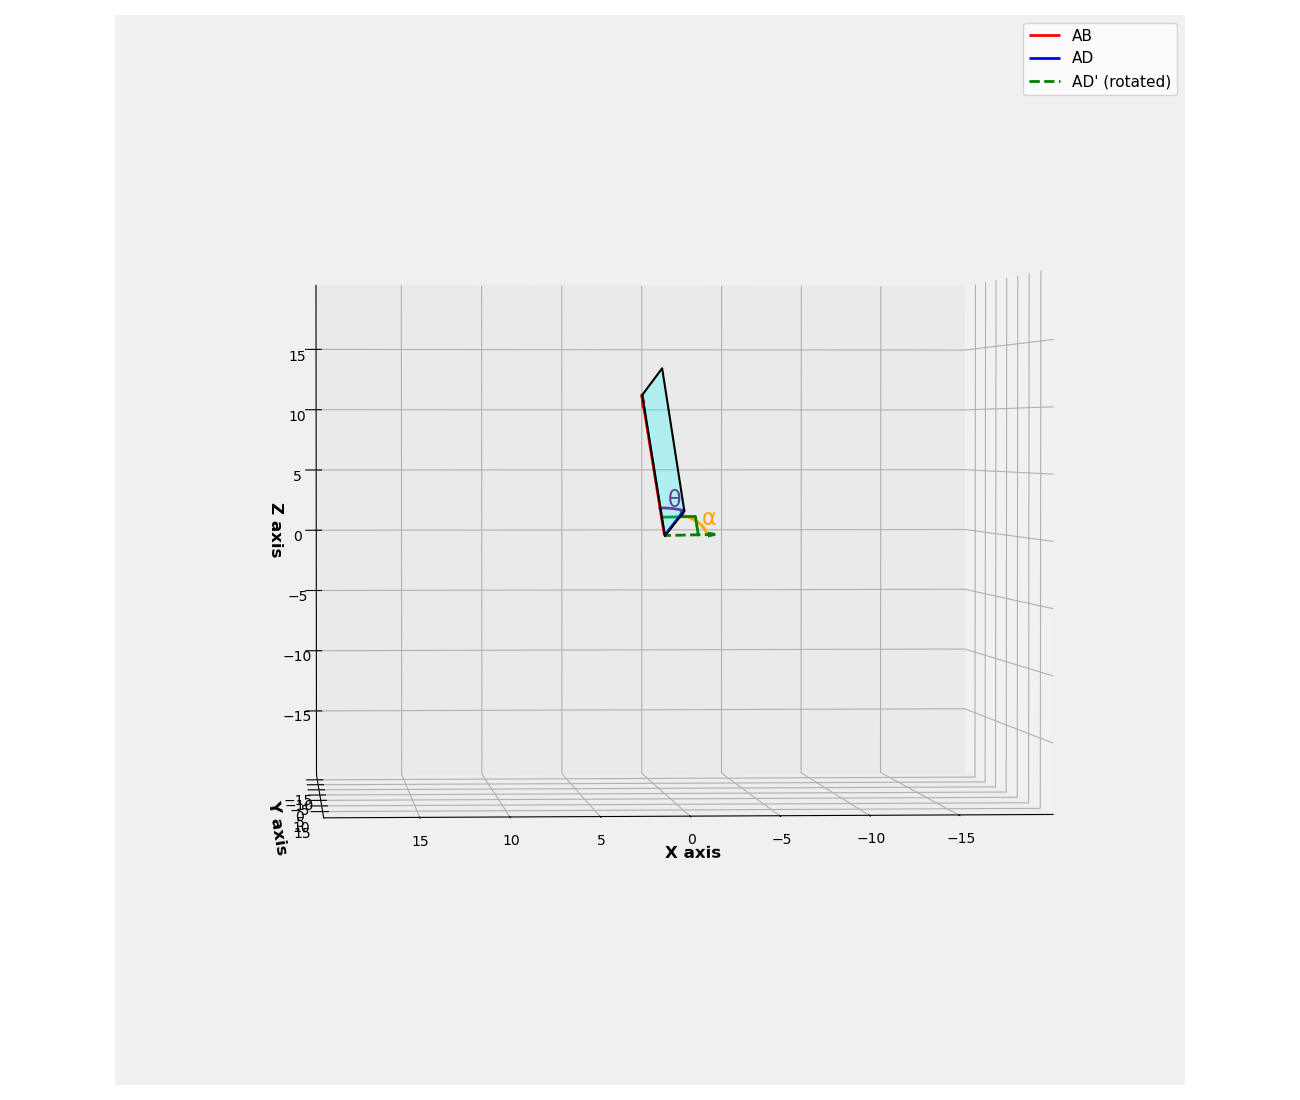
\includegraphics[width=1\columnwidth]{figs/plot2.png}
     \caption{Plot of the lines}
   \label{fig:placeholder_1}
\end{figure}

 \end{document}